\documentclass[10pt]{article}

\usepackage[letterpaper]{geometry}
\usepackage{enumerate,verbatim,mdwlist}
\usepackage{fancyhdr}
\usepackage{linguex}
\usepackage[colorlinks=true,linkcolor=blue]{hyperref}

%Packages needed for trees
\usepackage{amsfonts,amsmath,amssymb}
\usepackage[varg]{txfonts}
\usepackage{qtree}

%%%%%%%%%%%%%%%%%%%%%%%%%%%%%%%%%%%%%%%%%%%%%
%% Represent categorical logic graphically %%
%%%%%%%%%%%%%%%%%%%%%%%%%%%%%%%%%%%%%%%%%%%%%

\usepackage{tikz}
\usepackage{xstring}

\usetikzlibrary{shapes,backgrounds}
\tikzstyle{every node}=[font=\tiny] 

%%%%%%%%%%%%%%%%%%%%%%%%%%%%%%%%
%% Draw squares of Opposition %%
%%%%%%%%%%%%%%%%%%%%%%%%%%%%%%%%

\def\oppsquare{(-1.5,1) node[above left]{$All$} -- (1.5,1) node[above right]{$No$} -- (1.5,-1) node[below right]{$Some-not$} -- (-1.5,-1) node[below left]{$Some$} -- (-1.5,1)}
\def\oppcross{(-1.5,1) -- (1.5,-1) node[sloped,above,pos=0.3]{contra} node[sloped,above,pos=0.7]{dictory} (-1.5,-1) -- (1.5,1) node[sloped,above,pos=0.3]{contra} node[sloped,above,pos=0.7]{dictory}}

\def\sqroppMod{%
  \begin{scope}
    \draw \oppsquare;
    \draw \oppcross;
    \draw (-1.75,0) node[rotate=90] {undet.};
    \draw (0,1.25) node {undet.};
    \draw (0,-1.25) node {undet.};
    \draw (1.75,0) node[rotate=90] {undet.};
  \end{scope}
}

\def\sqroppTrad{%
  \begin{scope}
    \draw \oppsquare;
    \draw \oppcross;
    \draw (-1.75,0) node[rotate=90] {subalt.};
    \draw (0,1.25) node {contrary};
    \draw (0,-1.25) node {subcontrary};
    \draw (1.75,0) node[rotate=90] {subalt.};
  \end{scope}
}

%%%%%%%%%%% Turn categorical props into Venn diagrams %%%%%%%%%%%%%%%
%% \catvenn{title:<y/n>}{quantifier:<All/No/Some>}{quality:<not/>} %%
%%         {complement:<non-/>}{subject class}                     %%
%%         {complement:<non-/>}{predicate class}                   %%
%%%%%%%%%%%%%%%%%%%%%%%%%%%%%%%%%%%%%%%%%%%%%%%%%%%%%%%%%%%%%%%%%%%%%

%%%%%%%%%%%%%
%% Circles %%
%%%%%%%%%%%%%

%% Venn circles
\def\firstcircle{(0,0) circle (1cm)} 
\def\secondcircle{(0:1.5cm) circle (1cm)}
\def\thirdcircle{(60:1.5cm) circle (1cm)}

%% Overlapping and disjoint circles
\def\firstcircleN{(0,0) circle (.75cm) node [below left=.25in] {$A$}}
\def\secondcircleN{(0:2cm) circle (.75cm) node [below right=.25in] {$B$}}
\def\firstcircleA{(0,0) circle (1.25cm) node [above right] {$A$}}
\def\secondcircleA{(.125,0) circle (.75cm) node [below left=.25in] {$B$}}

%%%%%%%%%%%%%%%%%%%%%%%%%%%
%% Venn diagram template %%
%%%%%%%%%%%%%%%%%%%%%%%%%%%

\newcommand{\vennbox}[2]{%
  \draw (-1.5,-1.5) rectangle (3,1.5);
  \draw \firstcircle node [below left=.25in] {#1};
  \draw \secondcircle node [below right=.25in] {#2};
}

\newcommand{\syllbox}[3]{%
  \draw (-1.5,-1.5) rectangle (3,2.75);
  \draw \firstcircle node [below left=.25in] {#1};
  \draw \secondcircle node [below right=.25in] {#2};
  \draw \thirdcircle node [above right=.25in] {#3};
}

%%%%%%%%%%%%%%%%%%%%
%% Universal Defs %%
%%%%%%%%%%%%%%%%%%%%

\def\fillleft{%
  \begin{scope}[even odd rule, fill opacity=0.5]
    \clip \secondcircle (-1,-1) rectangle (1,1);
    \fill[blue] \firstcircle;
  \end{scope}
}

\def\fillmiddle{%
  \begin{scope}[fill opacity=0.5]
    \clip \firstcircle;
    \fill[blue] \secondcircle;
  \end{scope}
}

\def\fillright{%
  \begin{scope}[even odd rule, fill opacity=0.5]
    \clip \firstcircle (-1,-1) rectangle (2.5,1);
    \fill[blue] \secondcircle;
  \end{scope}
}

\def\fillbox{%
  \begin{scope}
    \fill[fill opacity=0.5, blue] (-1.5,-1.5) rectangle (3,1.5);
    \fill[fill opacity=1, white] \firstcircle \secondcircle;
  \end{scope}
}

%%%%%%%%%%%%%%%%%%%%%%
%% Existential Defs %%
%%%%%%%%%%%%%%%%%%%%%%

\def\xleft{%
  \node {x};
}
\def\xleftA{%
\draw (0,0) node [draw,rounded corners] {x};
}%

\def\xmiddle{%
  \node [right=.6cm] {x};
}
\def\xmidA{%
  \draw (.75cm,0) node [draw,rounded corners] {x};
}%

\def\xright{%
  \node [right=1.5cm] {x};
}

\def\xbox{%
 \node [below right=1.1cm] {x};
}

%%%%%%%%%%%%%%%%%%%
%% Draw diagrams %%
%%%%%%%%%%%%%%%%%%%

\newcommand{\catvenn}[7]{%
  \IfEqCase{#2}{%
    {All}{%
      \IfEqCase{#4}{%
	{non-}{%
	  \IfEqCase{#6}{%
	    {non-}{\fillright}%
	    {}{\fillbox}%
	  }[\PackageError{catvenn}{Undefined option to tree: pred-non}{}]%
	}%
	{}{%
	  \IfEqCase{#6}{%
	    {non-}{\fillmiddle}%
	    {}{\fillleft}%
	  }[\PackageError{catvenn}{Undefined option to tree: pred-non}{}]%
	}%
      }[\PackageError{catvenn}{Undefined option to tree: subj-non}{}]%
    }%
    {No}{%
      \IfEqCase{#4}{%
	{non-}{%
	  \IfEqCase{#6}{%
	    {non-}{\fillbox}%
	    {}{\fillright}%
	  }[\PackageError{catvenn}{Undefined option to tree: pred-non}{}]%
	}%
	{}{%
	  \IfEqCase{#6}{%
	    {non-}{\fillleft}%
	    {}{\fillmiddle}%
	  }[\PackageError{catvenn}{Undefined option to tree: pred-non}{}]%
	}%
      }[\PackageError{catvenn}{Undefined option to tree: subj-non}{}]%
    }%
    {Some}{%
      \IfEqCase{#3}{%
	{not}{%
	  \IfEqCase{#4}{%
	    {non-}{%
	      \IfEqCase{#6}{%
		{non-}{\xright}%
		{}{\xbox}%
	      }[\PackageError{catvenn}{Undefined option to tree: pred-non}{}]%
	    }%
	    {}{%
	      \IfEqCase{#6}{%
		{non-}{\xmiddle}%
		{}{\xleft}%
	      }[\PackageError{catvenn}{Undefined option to tree: pred-non}{}]%
	    }%
	  }[\PackageError{catvenn}{Undefined option to tree: subj-non}{}]%
	}%
	{}{%
	  \IfEqCase{#4}{%
	    {non-}{%
	      \IfEqCase{#6}{%
		{non-}{\xbox}%
		{}{\xright}%
	      }[\PackageError{catvenn}{Undefined option to tree: pred-non}{}]%
	    }%
	    {}{%
	      \IfEqCase{#6}{%
		{non-}{\xleft}%
		{}{\xmiddle}%
	      }[\PackageError{catvenn}{Undefined option to tree: pred-non}{}]%
	    }%
	  }[\PackageError{catvenn}{Undefined option to tree: subj-non}{}]%
	}%
      }[\PackageError{catvenn}{Undefined option to tree: not}{}]%
    }%
  }[\PackageError{catvenn}{Undefined option to tree: quant}{}]%
  
  \IfEqCase{#1}{%
    {y}{\draw (0,1.25) node {#2 #4#5 are #3 #6#7};}%
    {n}{}%
  }[\PackageError{catvenn}{Undefined option to tree: title}{}]%
  
  \vennbox{#5}{#7}%
}%

%%%%%%%%%%%%%%%%%%%%%%%%%%%%
%% Categorical syllogisms %%
%%%%%%%%%%%%%%%%%%%%%%%%%%%%

\newcommand{\filltopleft}[1]{%
  \begin{scope}[fill opacity=0.5]
    \clip \firstcircle;
    \fill[#1] \thirdcircle;
  \end{scope}
}

\newcommand{\filltopright}[1]{%
  \begin{scope}[fill opacity=0.5]
    \clip \secondcircle;
    \fill[#1] \thirdcircle;
  \end{scope}
}

\def\filltopfirst{%
  \begin{scope}[even odd rule, fill opacity=0.5]
    \clip \firstcircle (-1.5,-1.5) rectangle (3,2.75);
    \fill[green] \thirdcircle;
  \end{scope}
}

\def\filltopsecond{%
  \begin{scope}[even odd rule, fill opacity=0.5]
    \clip \secondcircle (-1.5,-1.5) rectangle (3,2.75);
    \fill[green] \thirdcircle;
  \end{scope}
}

\def\xtopleft{%
  \draw (60:.75cm) node [text=red] {x};
}

\def\xtopright{%
  \draw (30:1.3cm) node {x};
}

\def\xtopmid{%
  \draw (30:.85cm) node [text=red] {X};
}



%% Margin Setting
\geometry{hmargin={.5in,.5in},vmargin={1in,1in}}
\setlength{\parindent}{0.0in}
%\setlength{\parskip}{2mm}
\setlength{\tabcolsep}{10pt}
\setlength{\arraycolsep}{10pt}

%% Header
\setlength{\headheight}{23pt}
\pagestyle{fancy}
\fancyhead{}
\fancyhead[L]{Phil 101, f14}
\fancyhead[C]{Homework \# 3}
\fancyhead[R]{Due: Thursday October 16, 2014 \\ Point total: 20 points}

\begin{document}

\small

\textbf{Name:}\underline{\hspace{2in}}

\paragraph{The language of categorical logic}

\begin{enumerate}
 \item What is the primary difference between the \textbf{Boolean} and \textbf{Aristotelian} perspectives on categorical logic? \textbf{(1 point)}
 
\suspend{enumerate}

\vspace{1.5cm}

\paragraph{Syntactic relations}

\resume{enumerate}
  \item Write the converse of \textit{Some A are non-B}: \underline{\hspace{3in}} \textbf{(1 point)}
  
  \item Write the obverse of \textit{No Q are S}: \underline{\hspace{3in}} \textbf{(1 point)}
  
  \item Write the contraposition of \textit{Some non-M are not N}: \underline{\hspace{3in}} \textbf{(1 point)}
\suspend{enumerate}

\paragraph{Semantic relations}

\resume{enumerate}
  \item Assume that \textit{All A are B} is true. 
  
  Then the truth value of \textit{No A are B} is: \hspace{1cm} True \hspace{1cm} False \hspace{1cm} Undetermined \hspace{1cm} \textbf{(circle one, 1 point)} \\
  
  The relation that allows us to make that claim is: \underline{\hspace{3in}} \textbf{(1 point)}
  
  \item Assume that \textit{Some F are G} is false. 
  
  Then the truth value of \textit{All F are G} is: \hspace{1cm} True \hspace{1cm} False \hspace{1cm} Undetermined \hspace{1cm} \textbf{(circle one, 1 point)} \\
  
  The relation that allows us to make that claim is: \underline{\hspace{3in}} \textbf{(1 point)}
  
\suspend{enumerate}

\paragraph{Direct inferences}

\resume{enumerate}
  \item Assume the \textbf{Boolean perspective}, and consider the direct inference: \textit{Some W are not X}. Therefore, it is false that \textit{no W are X}.
  
  \vspace{3mm}
  
  This inference is: \hspace{1cm} Valid \hspace{1cm} Invalid \hspace{1cm} Conditionally valid \hspace{1cm} \textbf{(circle one, 1 point)}
  
  \vspace{3mm}
  
  Justify your answer in the space below.  You may use either method for assessing the validity of direct inferences. \textbf{(2 points)}
  
  \vspace{4cm}
  
  \item Assume the \textbf{Aristotelian perspective}, and consider the direct inference: It is false that \textit{some R are S}. Therefore, it is false that \textit{All R are S}.
  
  \vspace{3mm}
  
  This inference is: \hspace{1cm} Valid \hspace{1cm} Invalid \hspace{1cm} Conditionally valid \hspace{1cm} \textbf{(circle one, 1 point)}
  
  \vspace{3mm}
  
  Justify your answer in the space below.  You may use either method for assessing the validity of direct inferences. \textbf{(2 points)}
  
\suspend{enumerate}

\newpage

\paragraph{Syllogisms}

\resume{enumerate}
  \item Consider the syllogism:
    \begin{enumerate}[1)]
     \item All P are M
     \item All M are S
     \item $\therefore,$ some S are P
    \end{enumerate}

    This syllogism is: \hspace{1cm} Valid \hspace{1cm} Invalid \hspace{1cm} Conditionally valid \hspace{1cm} \textbf{(circle one, 1 point)}
    
    \vspace{3mm}
    
    Justify your answer using the Venn diagram below \textbf{(2 points)}
    
    \begin{center}
    \begin{tikzpicture}
     \syllbox{S}{P}{M}
    \end{tikzpicture}
    \end{center}

  \item Consider the syllogism:
    \begin{enumerate}[1)]
     \item Some M are P
     \item No S are M
     \item $\therefore,$ some S are not P
    \end{enumerate}

    This syllogism is: \hspace{1cm} Valid \hspace{1cm} Invalid \hspace{1cm} Conditionally valid \hspace{1cm} \textbf{(circle one, 1 point)}
    
    \vspace{3mm}
    
    Justify your answer using the Venn diagram below \textbf{(2 points)}
    
    \begin{center}
    \begin{tikzpicture}
     \syllbox{S}{P}{M}
    \end{tikzpicture}
    \end{center}
  
\end{enumerate}
  
\paragraph{Bonus:}  Demonstrate the fact that \textit{All Y are Z} and its obverse always have the same truth value. \textbf{(3 points)}

\end{document}
